\documentclass[a4paper, 12pt]{article}%тип документа

%%%Библиотеки
	%\usepackage[warn]{mathtext}	
	\usepackage[T2A]{fontenc} % кодировка
	\usepackage[utf8]{inputenc} % кодировка исходного текста
	\usepackage[english,russian]{babel} % локализация и переносы
	\usepackage{caption}
	\usepackage{listings}
	\usepackage{amsmath,amsfonts,amssymb,amsthm,mathtools}
	\usepackage{wasysym}
	\usepackage{graphicx}%Вставка картинок правильная
	\usepackage{float}%"Плавающие" картинки
	\usepackage{wrapfig}%Обтекание фигур (таблиц, картинок и прочего)
	\usepackage{fancyhdr} %загрузим пакет
	\usepackage{lscape}
	\usepackage{xcolor}
	\usepackage[normalem]{ulem}
	\usepackage{hyperref}

%%%Конец библиотек




%%%Настройка ссылок
	\hypersetup
	{
		colorlinks=true,
		linkcolor=blue,
		filecolor=magenta,
		urlcolor=blue
	}
%%%Конец настройки ссылок


%%%Настройка колонтитулы
	\pagestyle{fancy}
	\fancyhead{}
	\fancyhead[L]{Лабораторная работа}
	\fancyhead[R]{Талашкевич Даниил, группа Б01-009}
	\fancyfoot[C]{\thepage}
%%%конец настройки колонтитулы



							\begin{document}
						%%%%Начало документа%%%%


%%%Начало титульника
\begin{titlepage}

	\newpage
	\begin{center}
		\normalsize Московский физико-технический институт \\(госудраственный 			университет)
	\end{center}

	\vspace{6em}

	\begin{center}
		\Large Лабораторная работа по электричеству\\
	\end{center}

	\vspace{1em}

	\begin{center}
		\large \textbf{Спектры электрических сигналов (компьютер) [3.6.1]}
	\end{center}

	\vspace{2em}

	\begin{center}
		\large Талашкевич Даниил Александрович\\
		Группа Б01-009
	\end{center}

	\vspace{\fill}

	\begin{center}
	Долгопрудный \\2021
	\end{center}
	
\end{titlepage}
%%%Конец Титульника



%%%Настройка оглавления и нумерации страниц
	\thispagestyle{empty}
	\newpage
	\tableofcontents
	\newpage
	\setcounter{page}{1}
%%%Настройка оглавления и нумерации страниц


					%%%%%%Начало работы с текстом%%%%%%

\section{Аннотация}

В работе изучается спектральный состав периодических электрических сигналов различной формы: последовательности прямоугольных импульсов, последовательности цугов и амплитудно модулированных гармонических колебаний. Спектры этих сигналов наблюдаются с помощью промышленного анализатора спектра и сравниваются с рассчитанными теоретически. 

\section{Теоретические сведения}

Сколь угодно сложныи электрическии сигнал $\mathrm{V}$ (t) может быть разложен на более простые сигналы. В радиотехнике широко используется разложение сигнала V (t) на совокупность гармонических сигналов различных частот $\omega .$ Функция $\mathrm{F}(\omega)$, описывающая зависимость амплитуд отдельных гармоник от частоты, называется амплитуднои спектральнои характеристикои сигнала $\mathrm{V}(\mathrm{t})$. Представление сложного периодического сигнала в виде суммы дискретных гармонических сигналов в математике называется разложением в ряд Фурье.

Зная спектральныи состав $\mathrm{F}(\omega)$ периодическои последовательности некоторого импульса V (t), мы можем осуществить обратное преобразование Фурье: сложив отдельные гармоники со своими амплитудами и фазами, получить необходимую последовательность импульсов. Степень совпадения полученного сигнала с V (t) определяется количеством синтезированных гармоник: чем их больше, тем лучше совпадение.
Рассмотрим конкретные примеры периодических функции, которые будут предметом исследования в нашеи работе.

Рассмотрим конкретные примеры периодических функций, которые будут предметом исследования в нашей работе.

\subsection{Спектральный анализ электрических сигналов}

\begin{center}
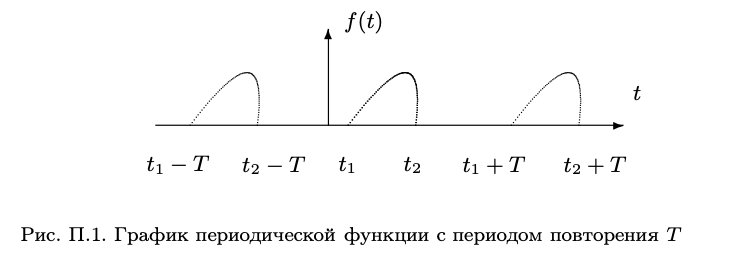
\includegraphics[width=0.7\linewidth]{./anat/1.jpg}\\
\end{center}

Пусть заданная функция $f(t)$ периодически повторяется с частотой $\Omega_{1}=2 \pi / T,$ где $T-$ период повторения $($ рис. $\Pi .1) .$ Её разложение в ряд Фурье имеет вид
$$
f(t)=\frac{a_{0}}{2}+\sum_{n=1}^{\infty}\left[a_{n} \cos \left(n \Omega_{1} t\right)+b_{n} \sin \left(n \Omega_{1} t\right)\right]
$$
или
$$
f(t)=\frac{A_{0}}{2}+\sum_{n=1}^{\infty} A_{n} \cos \left(n \Omega_{1} t-\psi_{n}\right)
$$
Здесь $a_{0} / 2=A_{0} / 2-$ постоянная составляюпдая (среднее значение) функции $f(t) ; a_{n}$ и $b_{n}-$ амплитуды косинусных и синусных членов разложе-ния. Они определяются выражениями
$$
\begin{array}{l}
a_{n}=\frac{2}{T} \int_{t_{1}}^{t_{1}+T} f(t) \cos \left(n \Omega_{1} t\right) d t \\
b_{n}=\frac{2}{T} \int_{t_{1}}^{t_{1}+T} f(t) \sin \left(n \Omega_{1} t\right) d t
\end{array}
$$

Точку начала интегрирования $t_{1}$ можно выбрать произвольно. В тех случаях, когда сигнал четен относительно $\mathrm{t}=0$, в тригонометрическои записи остаются только косинусные члены, т.к. все коэффициенты $b_{n}$ обращаются в нуль. Для нечетнои относительно $\mathrm{t}=0$ функции, наоборот, ряд состоит только из синусных членов.

Амплитуда $A_{n}$ и фаза $\psi_{n} n$ -й гармоники выражаются через $a_{n}$ и $b_{n}$ следуюшим образом:
$$
A_{n}=\sqrt{a_{n}^{2}+b_{n}^{2}} ; \quad \psi_{n}=\operatorname{arctg} \frac{b_{n}}{a_{n}}
$$
Как мы видим, спектр любой периодической функции состоит из набора гармонических колебаний с дискретными частотами: $\Omega_{1}, 2 \Omega_{1}, 3 \Omega_{1}$ $\ldots$ и постоянной составляющей, которую можно рассматривать как колебание с нулевой частотой $\left(0 \cdot \Omega_{1}\right) .$

Представим выражение в комплексной форме. Для этого заменим косинусы экспонентами в соответствии с формулой
$$
\cos \alpha=\frac{e^{i \alpha}+e^{-i \alpha}}{2}
$$
Подстановка даёт
$$
f(t)=\frac{1}{2}\left(A_{0}+\sum_{n=1}^{\infty} A_{n} e^{-i \psi_{n}} e^{i n \Omega_{1} t}+\sum_{n=1}^{\infty} A_{n} e^{i \psi_{n}} e^{-i n \Omega_{1} t}\right)
$$
Введём комплексные амплитуды $\tilde{A}_{n}$ и $\tilde{A}_{-n}$

$$
\tilde{A}_{n}=A_{n} e^{-i \psi_{n}} ; \quad \tilde{A}_{-n}=A_{n} e^{i \psi_{n}} ; \quad \tilde{A}_{0}=A_{0}
$$
Разложение $f(t)$ приобретает вид
$$
f(t)=\frac{1}{2} \sum_{n=-\infty}^{\infty} \tilde{A}_{n} e^{i n \Omega_{1} t}
$$

Как мы видим, введение отрицательных частот (типа $\mathrm{n} \Omega_{1}$ ) позволяет записать разложение Фурье особенно поостым образом.

Для расчёта комплексных амплитуд $A_{n}$ yмножим левую и правую части на $e^{-i k \Omega_{1} t}$ и проинтегрируем полученное равенство по времени на отрезке, равном одному периоду, например, от $t_{1}=0$ до $t_{2}=2 \pi / \Omega_{1} .$ В правой части обратятся в нуль все члены, кроме одного, соответствующего $n=k .$ Этот член даёт $A_{k} T / 2 .$ Имеем поэтому
$$
A_{k}=\frac{2}{T} \int_{0}^{T} f(t) e^{-i k \Omega_{1} t} d t
$$
Рассмотрим периодические функции, которые исследуются в нашей paбoтe.


\subsection{Периодическая последовательность прямоугольных импульсов}
C амплитудой $V_{0},$ длительностью $\tau,$ частотой повторения $f_{\text {повт }}=1 / T,$ где $T-$ период повторения импульсов.


Cреднее значение

$\langle V\rangle=\frac{a_{0}}{2}=\frac{A_{0}}{2}=\frac{1}{T} \int_{-\tau / 2}^{\tau / 2} V_{0} d t=V_{0} \frac{\tau}{T}$

Амплитуды косинусных составляющих равны

$$
a_{n}=\frac{2}{T} \int_{-\tau / 2}^{\tau / 2} V_{0} \cos \left(n \Omega_{1} t\right) d t=2 V_{0} \frac{\tau}{T} \frac{\sin \left(n \Omega_{1} \tau / 2\right)}{n \Omega_{1} \tau / 2} \sim \frac{\sin x}{x}
$$
Поскольку наша функция чётная, все амплитуды синусоидальных гармоник $b_{n}=0 .$ Спектр $F(\nu)$ последовательности прямоугольных импульсов представлен на рис. П.3. Амплитуды гармоник $A_{n}$ меняются по Закону $(\sin x) / x$
На рис. П.3 изображён спектр для случая, когда $T$ кратно $\tau .$ Назовём шириной спектра $\Delta \omega$ (или $\Delta \nu$ ) расстояние от главного максимума $(\nu=0)$ до первого нуля, возникающего, как нетрудно убедиться, при $\Omega_{1}=2 \pi / \tau$ При этом
$$
\Delta \omega \tau \simeq 2 \pi \quad \text { или } \quad \Delta \nu \Delta t \simeq 1
$$
Полученное соотношение взаимной связи интервалов $\Delta \nu$ и $\Delta t$ является
частным случаем соотношения неопределенности в квантовой механике. Несовместимость острой локализации волнового процесса во времени с узким спектром частот - явление широко известное в радиотехнике. Ширина селективной настройки $\Delta \nu$ радиоприёмника ограничивает приём радиосигналов Длительностью $t<1 / \Delta \nu$

 \begin{center}
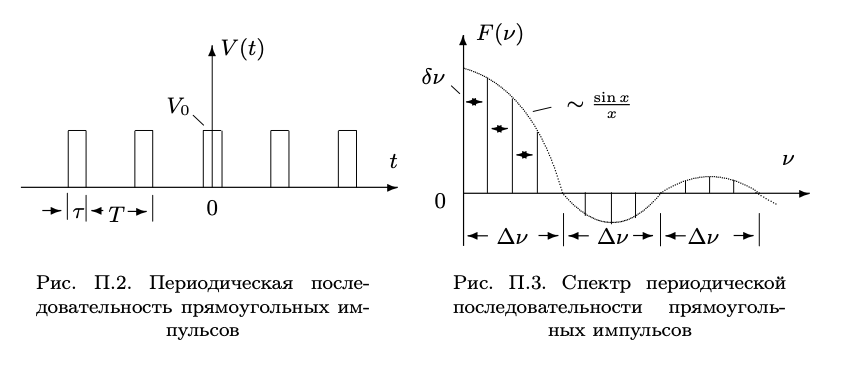
\includegraphics[width=0.7\linewidth]{./anat/2.jpg}\\
\end{center}

\subsection{Периодическая последовательность цугов}
Гармонического колебания $V_{0} \cos \left(\omega_{0} t\right)$ с длительностью цуга $\tau$ и периодом повторения $T$ (рис. $\Pi .4)$
 
Функция $f(t)$ снова является чётной относительно $t=0 .$ Амплитуда $n$ -й гармоники равна
$$
\begin{array}{c}
A_{n}=a_{n}=\frac{2}{T} \int_{-\tau / 2}^{\tau / 2} V_{0} \cos \left(\omega_{o} t\right) \cdot \cos \left(n \Omega_{1} t\right) d t= \\
=V_{0} \frac{\tau}{T}\left(\frac{\sin \left[\left(\omega_{0}-n \Omega_{1}\right) \frac{\tau}{2}\right]}{\left(\omega_{0}-n \Omega_{1}\right) \frac{\tau}{2}}+\frac{\sin \left[\left(\omega_{0}+n \Omega_{1}\right) \frac{\tau}{2}\right]}{\left(\omega_{0}+n \Omega_{1}\right) \frac{\tau}{2}}\right)
\end{array}
$$

Такое спектральное распределение F ($\omega$) для случая, когда $\frac T\tau$ равно целому числу, представлено на рис. П.5. Сравнивая спектр последовательности прямоугольных импульсов и спектр цугов (см. рис. П.3 и П.5), мы видим, что они аналогичны, но их максимумы сдвинуты по частоте на величину $\omega_0$.

\begin{center}
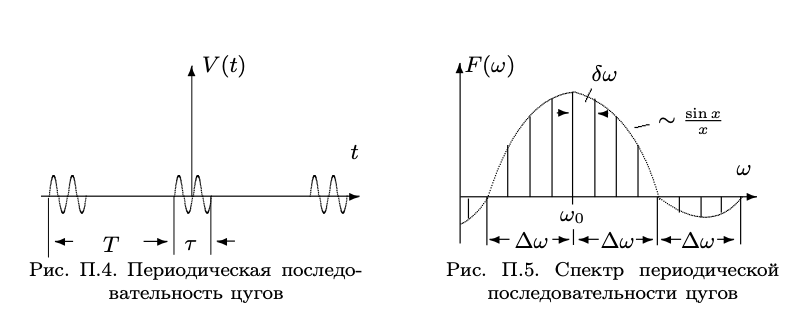
\includegraphics[width=0.7\linewidth]{./anat/3.jpg}\\
\end{center}

\subsection{Амплитудно-модулированные колебания.}

\begin{center}
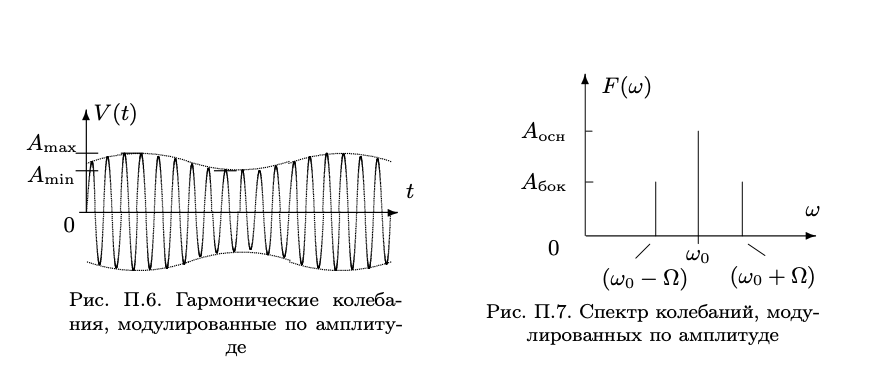
\includegraphics[width=0.7\linewidth]{./anat/4.jpg}\\
\end{center}
 Рассмотрим гармонические колебания высокой частоты $\omega_{0},$ амплитуда которых медленно меняется по гармоническому закону с частотой $\Omega\left(\Omega \ll \omega_{0}\right)$ (рис. П.6):
$$
f(t)=A_{0}[1+m \cos (\Omega t)] \cos (\omega t)
$$
Коэффициент $m$ называют глубиной модуляции. При $m<1$ амплитуда колебаний меняется от минимальной $A_{\min }=A_{0}(1-m)$ до максимальной $A_{\max }=A_{0}(1+m) .$ Глубина модулящии может быть представлена в виде
$$
m=\frac{A_{\max }-A_{\min }}{A_{\max }+A_{\min }}
$$
Простым тригонометрическим преобразованием можно найти спектр амплитудно-модулированных колебаний:
$$
\begin{aligned}
f(t) &=A_{0} \cos \left(\omega_{0} t\right)+A_{0} m \cos (\Omega t) \cos \left(\omega_{0} t\right)=\\
=A_{0} \cos \left(\omega_{0} t\right) &+\frac{A_{0} m}{2} \cos \left(\omega_{0}+\Omega\right) t+\frac{A_{0} m}{2} \cos \left(\omega_{0}-\Omega\right) t
\end{aligned}
$$

Спектр $F(\omega)$ таких колебаний содержит три составляюшцих (рис. П. 7$)$ Основная компонента представляет собой исходное немодулированное колебание с иесущей частотой $\omega_{0}$ и амплитудой $A_{\mathrm{ocн}}=A_{0}-$ первое слагаемое в правой части; боковые компоненты спектра соответствуют гармоническим колебаниям с частотами $\left(\omega_{0}+\Omega\right)$ и $\left(\omega_{0}-\Omega\right)-$ Второе и третье слагаемые. Амплитуды этих двух колебаний одинаковы и составляют $m / 2$ от амплитуды немодулированного колебания: $A_{\text {бок }}=A_{0} m / 2$


\section{Метод, результаты и обработка}

\subsection{Исследование спектра периодических последовательностей прямоугольных импульсов}
Устанавливаем прямоугольные колебания c $\nu_{\text{повт}} = 1$ кГц (период $T = 1$ мс) и длительностью импульса $\tau = 100$ мкс.

Получаем на экране спектр сигнала и, изменяя либо $\tau$, либо $\nu_{\text{повт}}$, наблюдаем, как изменяется спектр.

\begin{center}
\begin{tabular}{cc}
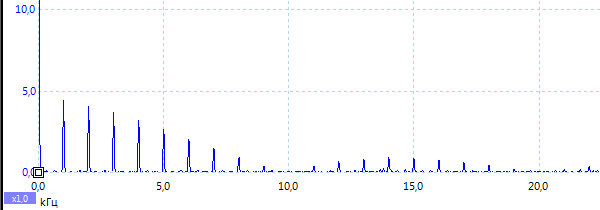
\includegraphics[width=0.45\textwidth]{./res/6.png}&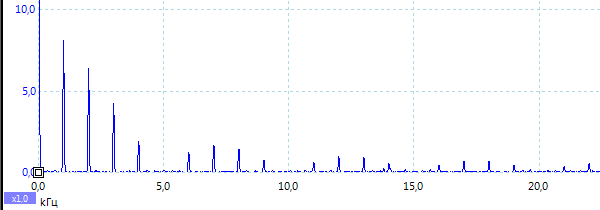
\includegraphics[width=0.45\textwidth]{./res/7a.png}\\

$\nu_{\text{повт}} = 1$ кГц, $\tau = 100$ мкс&$\nu_{\text{повт}} = 1$ кГц, $\tau = 200$ мкс\\

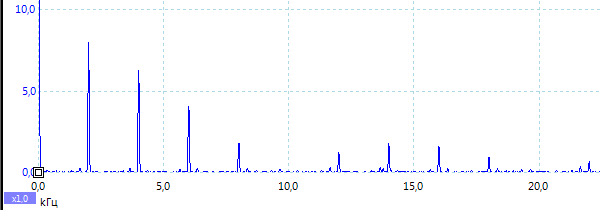
\includegraphics[width=0.45\textwidth]{./res/7b.png}\\

$\nu_{\text{повт}} = 2$ кГц, $\tau = 100$ мкс\\
\end{tabular}
\end{center}
Из данных видно, что, при увеличении $\tau$, уменьшается $\Delta \nu$, а при увеличении $\nu_\text{повт}$, увеличивается расстояние между пиками.

Измерим зависимость $\Delta \nu$ от $\tau$:
\begin{center}
\begin{tabular}{|c|c|c|c|c|}\hline
$\tau\text{, мкс}$&$\nu_0\text{, кГц}$&$\Delta \nu_0\text{, кГц}$&$1/\nu_0\text{, мкс}$&$\Delta 1/\nu_0\text{, мкс}$\\\hline
$40.0$&$30$&$30$&$40.0$&$0$\\\hline
$60.0$&$17$&$17$&$59$&$3$\\\hline
$80.0$&$13$&$13$&$77$&$6$\\\hline
$100.0$&$10$&$10$&$100.0$&$0$\\\hline
$120.0$&$8$&$8$&$125$&$16$\\\hline
$140.0$&$7$&$7$&$140$&$20$\\\hline
$160.0$&$6$&$6$&$170$&$30$\\\hline
$180.0$&$6$&$6$&$170$&$30$\\\hline
$200.0$&$5$&$5$&$200.0$&$0$\\\hline
\end{tabular}\\~\\
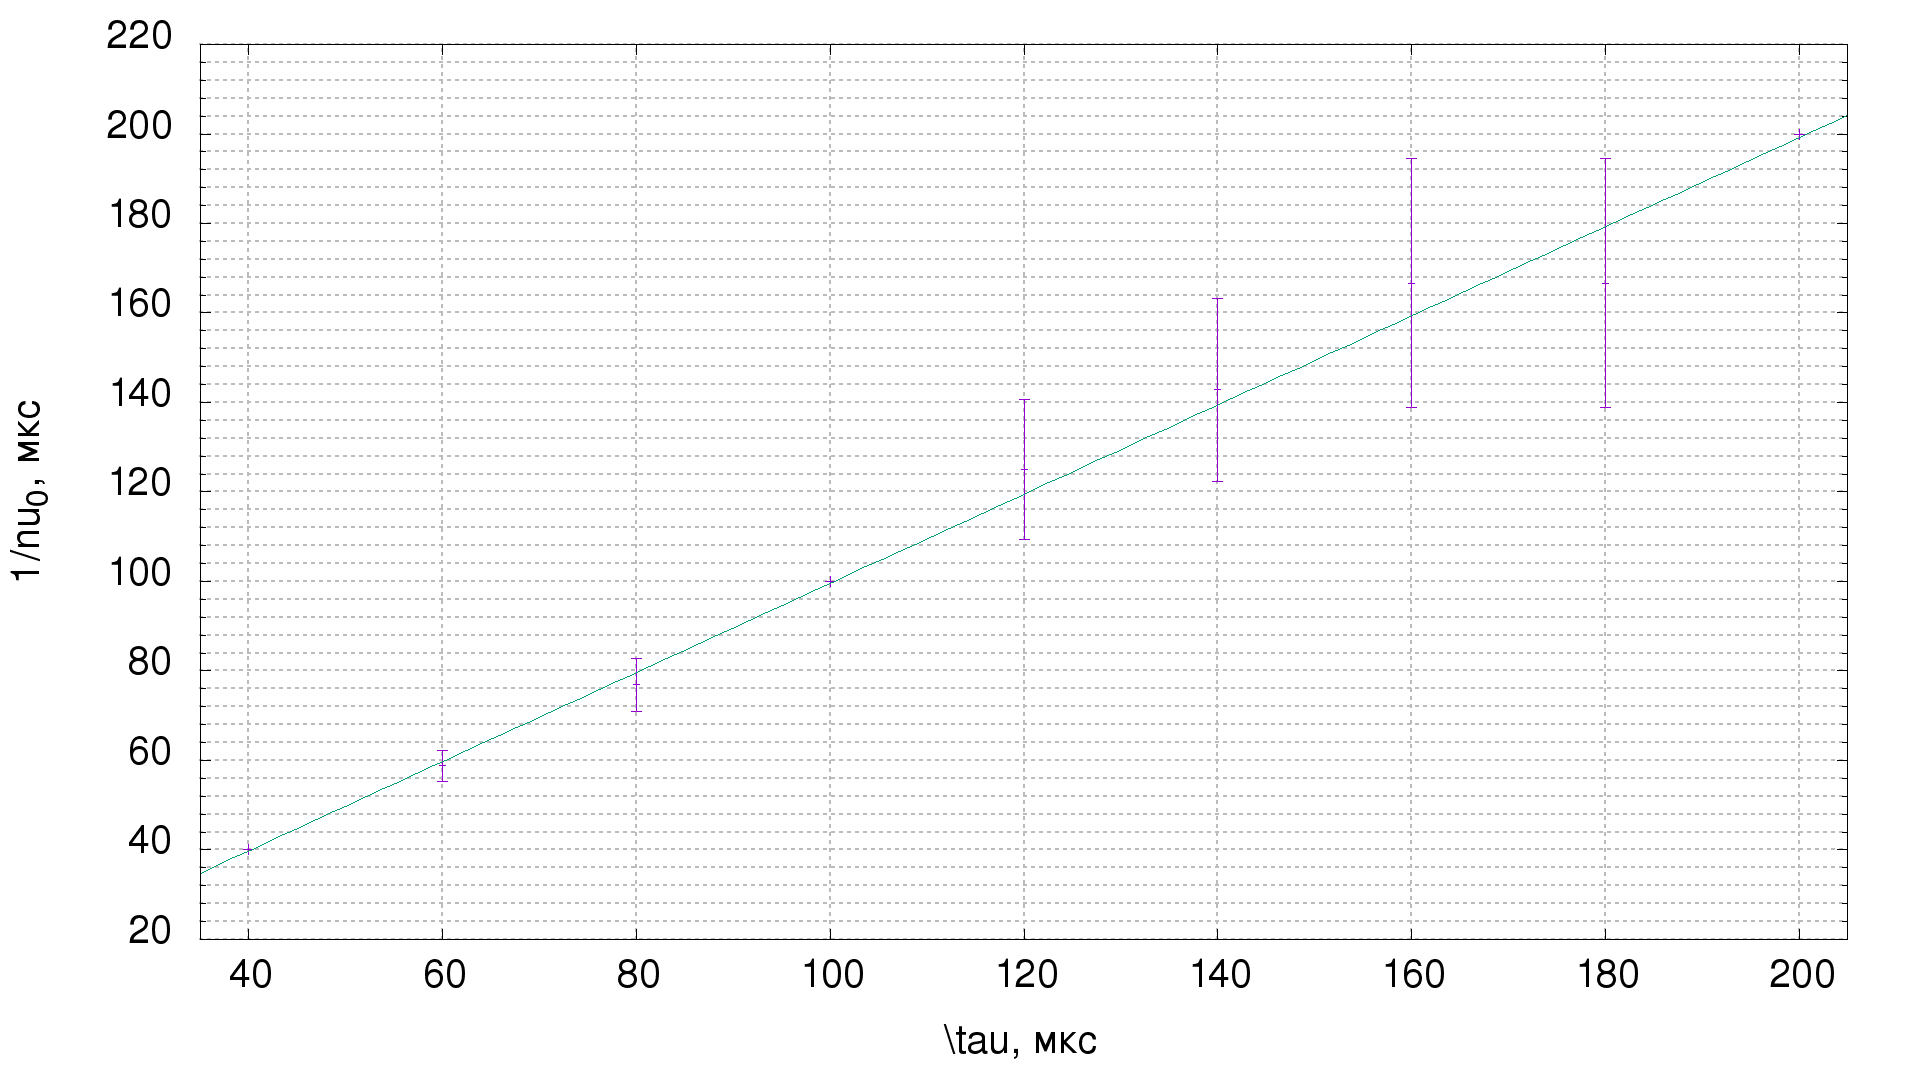
\includegraphics[width=0.95\textwidth]{./res/data.png}
\end{center}

Из графика $\Delta \nu \cdot \tau = 1.004\pm0.014$, что подтверждает соотношение неопределенностей.

\subsection{Исследование спектра периодической последовательности цугов}
Посмотрим на последовательность цугов с характерными параметрами: $\nu_0 = 50$ кГц частота повторения импульсов $f_\text{повт}=1$ кГц и исследуем спектр этого сигнала для разных длительностей импульса:
\begin{center}
\begin{tabular}{cc}
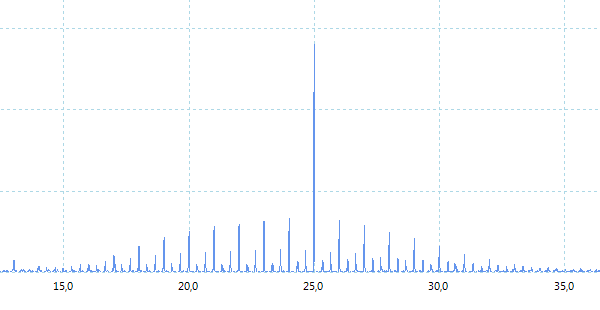
\includegraphics[width=0.45\textwidth]{./res/100_pulse.png}&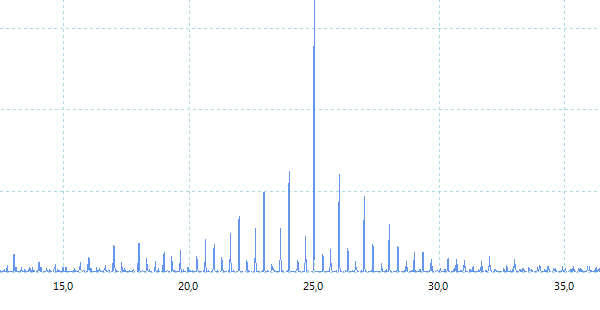
\includegraphics[width=0.45\textwidth]{./res/200_pulse.png}\\
$\tau = 100$ мкс&$\tau = 200$ мкс\\
\end{tabular}
\end{center}
Из данных видно, что при изменении $\tau$ значение $\Delta \omega$ обратнопропорционально меняется.\\

Рассмотрим поведение спектрограммы при фиксировнном значении $\tau$ и меняющемся значении $\nu_0$:
\begin{center}
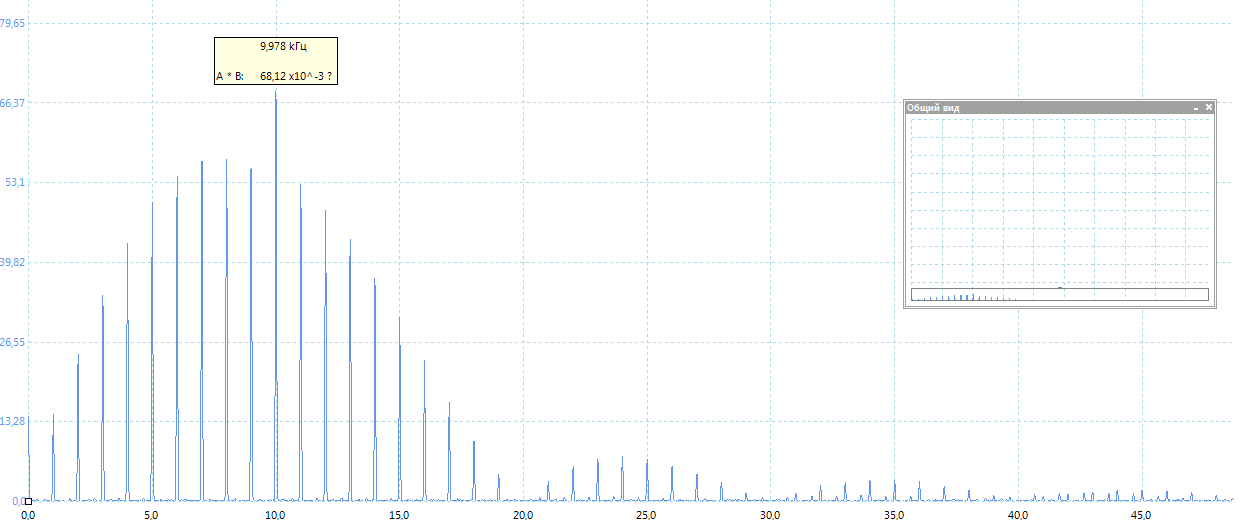
\includegraphics[width=0.95\textwidth]{./res/AB10.png}\\
$\nu_0=10$ кГц
\end{center}
\begin{center}
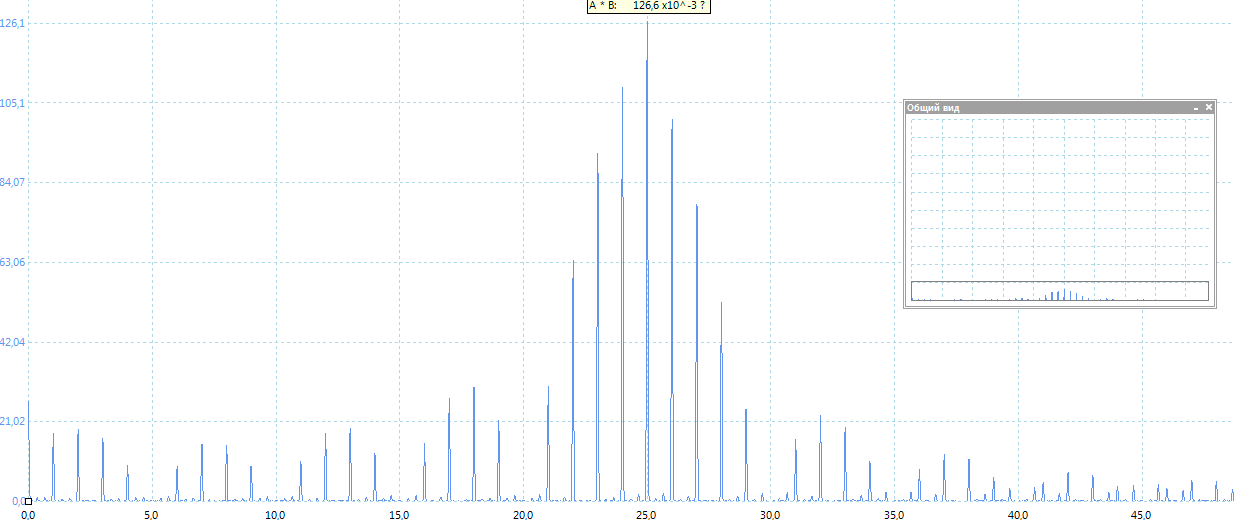
\includegraphics[width=0.95\textwidth]{./res/AB25.png}\\
$\nu_0=25$ кГц
\end{center}
\begin{center}
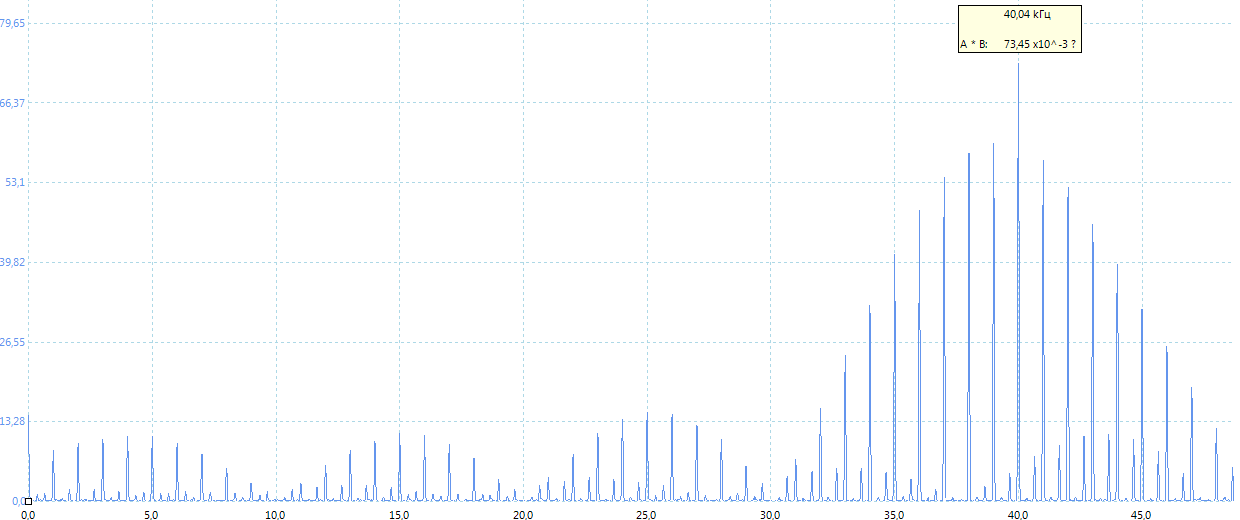
\includegraphics[width=0.95\textwidth]{./res/AB40.png}\\
$\nu_0=40$ кГц
\end{center}
Из данных видно, что при изменении $\nu_0$ картина смещается без изменения расстояния между спектральными компонентами.\\
Рассмотрим то, как это расстояние меняется при изменении $f_\text{повт}$:
\begin{center}
\begin{tabular}{|c|c|}\hline
$f_\text{повт}$&$\nu, \text{кГц}$\\\hline
$0.5$&$0.5$\\\hline
$1.0$&$1.0$\\\hline
$2.0$&$2.0$\\\hline
$4.0$&$4.0$\\\hline
$5.0$&$5.0$\\\hline
\end{tabular}\\~\\
\end{center}
Погрешность результатов определяется погрешностью генератора -- $0.5$ Гц.
$$\frac{f_\text{повт}}{\nu, \text{кГц}} = 1\pm0.1\%,$$
что согласуется с теорией.

\subsection{Исследование спектра амплитудно модулированного сигнала}
Рассмотрим амплитудно промодулированную синусоиду с параметрами $\nu_0=25$кГц, $\nu_\text{мод}=1$кГц:

\begin{center}
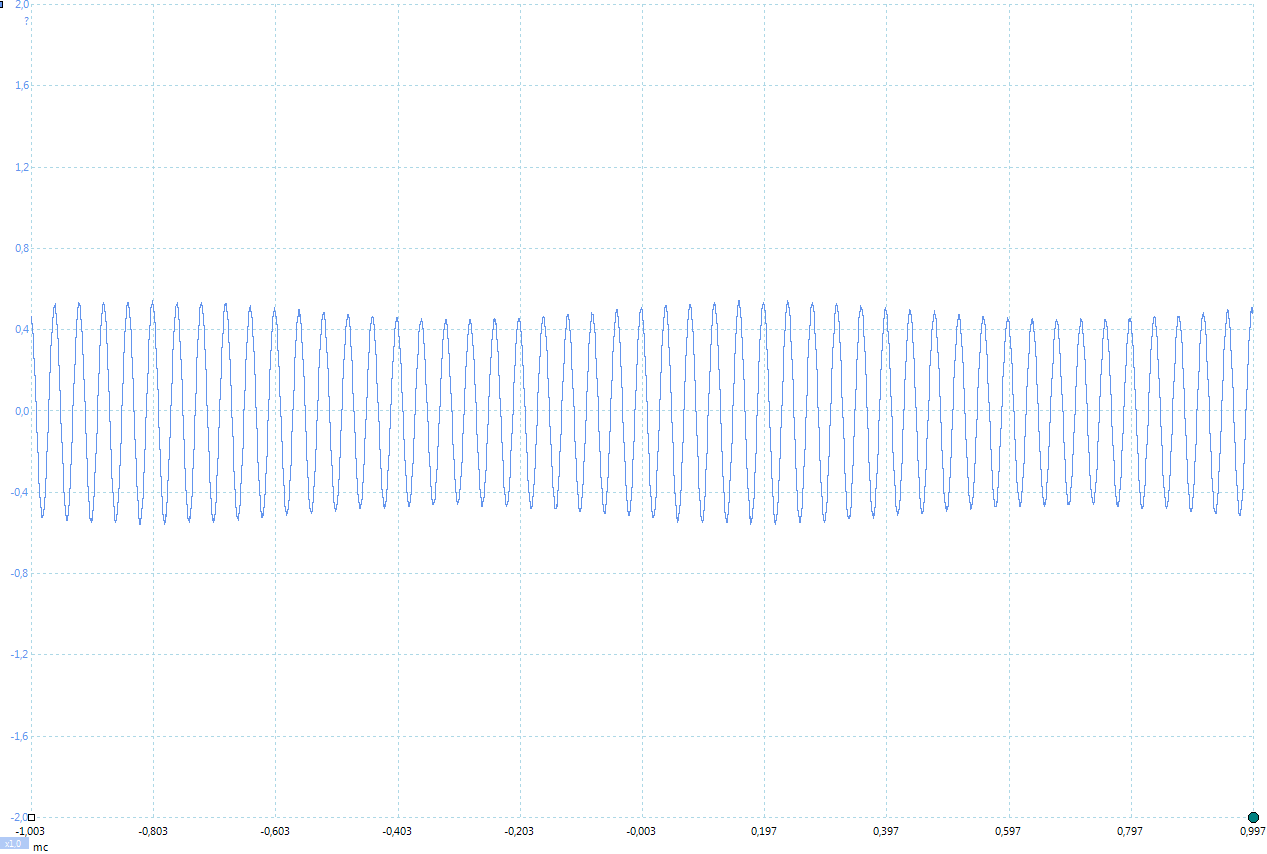
\includegraphics[width=0.95\textwidth]{./res/sin_mod.png}\\
$\nu_0=40$ кГц
\end{center}
\newpage
Посмотрим на спектрограмму этого сигнала:\\
<тут должен быть скрин со спектрограммой, но у меня его нет>
\begin{center}
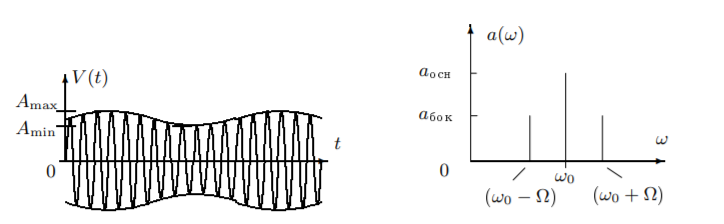
\includegraphics[scale=0.9]{./res/4.png}
\end{center}
Посмотрим зависимость отношения амплитуд $k=A_\text{бок}/A_\text{осн}$ у боковых и остовной частоты от параметра $m = (A_{max} - A_{min}) / (A_{max} + A_{min})$.
\begin{center}
\begin{tabular}{|c|c|c|c|}\hline
$A_{max}-A_{min}\text{, В}$&$A_\text{бок}\text{, В}$&$m$&$k$\\\hline
$0.2$&$0.0160$&$0.1$&$0.0497$\\\hline
$0.6$&$0.0470$&$0.3$&$0.1460$\\\hline
$1.0$&$0.0750$&$0.5$&$0.2329$\\\hline
$1.4$&$0.1070$&$0.7$&$0.3323$\\\hline
$1.8$&$0.1390$&$0.9$&$0.4317$\\\hline
$2.0$&$0.1530$&$1.0$&$0.4752$\\\hline
\end{tabular}\\~\\
$A_\text{осн} = (322\pm0.5)\text{мВ},\,\Delta A_\text{бок}=0.0005\,\text{В},\Delta k=0.0016\,\text{}$
\end{center}
\begin{center}
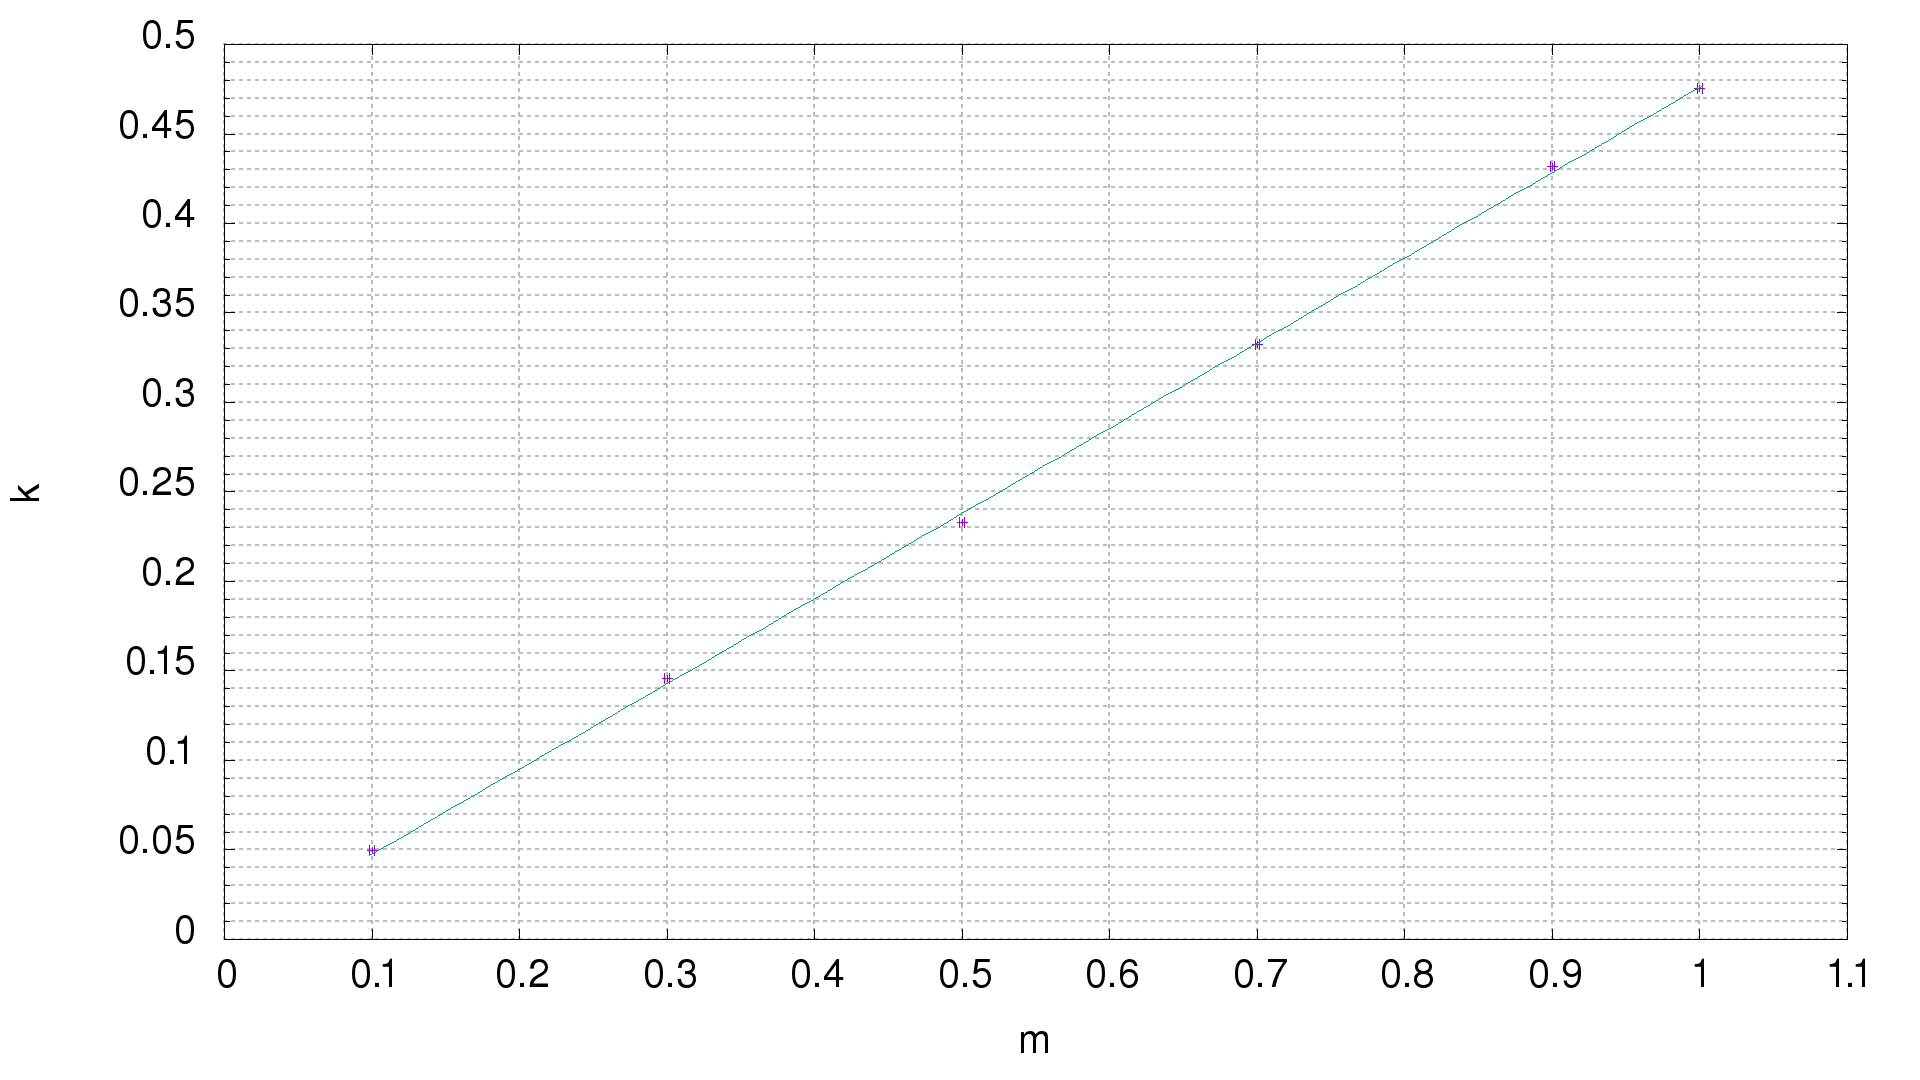
\includegraphics[width=0.95\textwidth]{./res/plot2.png}
\end{center}
Из графика
$$\frac{k}{m} = 0.476\pm0.015,$$
что сходится с теоретическим значением $0.5$.

\section{Вывод}

В данной работе мы изучили понятие спектра и ознакомились с принципами спектрального анализа, а также исследовали спектральный состав периодических электрических сигналов. 

Мы посмотрели на прямоугольные импульсы, цуги гармонических колебаний, а также гармонические сигналы, модулированные по амплитуде. Кроме того, был экспериментально проверен частный случай выполнения соотношения неопределённости. 

XX
 

\section{Литература}

\begin{enumerate}
\item \textbf{Лабораторный практикум по общей физике:} учеб. пособие. В трёх томах. Т. 2. Электричество и магнетизм /
Никулин М. Г., Попов П. В., Нозик А. А., и др.; под ред. А. В. Мак­симычева, М. Г. Никулина. — 2-е изд., перераб. и доп. — Москва : МФТИ, 2019. — 370 с.
ISBN 978-5-7417-0709-8 (Т. 2. Электричество и магнетизм)
\end{enumerate}		
		

\end{document}
